\addchap{Theory}

\section{Pumps}
\subsection{Rotary Vane Pump}
The rotary vane pump is a rotational displacement pump.
Inside of the outer casing, the so called stator, an excentrically mounted rotor is rotating.
Vanes are allowed to slide out of this rotor either spring-loadedly or by centrifugal force and are pressed permanently against the inner wall of the pump, effectively creating small chambers which do the pump work.
Lubrication is provided by grease, so the vanes always transport a small amount of lubricant to the outlet as well, which is fed back into the pump afterwards.
Lubrication oil ensures that the individual vane chambers are sealed properly, which increases effectivity.
The pump's suction effect is caused by the increasing volume of the vane chamber as the rotor rotates.
Pumped air is then compressed at the discharge side of the pump and expelled afterwards.
Rotary vane pumps are used to create a low-vacuum.
This experiment's apparatus features a two-staged rotary vane pump with vacuum-sided adsorption trap and discharge-sided exhaust filter.

\subsection{Turbomolecular Pump}
Turbomolecular pumps work on the principle that momentum is transmitted to gas molecules in a desired direction by repeatedly colliding with a moving solid surface.
In this type of pump, a series of rapidly rotating fans hit the gas molecules from the inlet of the pump towards the discharge side in order to create a vacuum.

As the gas molecules enter through the inlet, the rotor hits the molecules with a number of angled blades.
Thus the mechanical energy of the blades is transferred to the gas molecules.
With this newly acquired momentum, the gas molecules enter into the gas transfer holes in the stator.
This leads them to the next stage where they again collide with the rotor surface, this process is continued further, finally leading them outwards through the exhaust.

\section{Vakuum Gauges}
\subsection{Ion Gauge}
An ion gauge basicly consists of an electron emitting cathode, an anode and an ion collector.
The electrons emitted by the cathode are accelerated towards the anode and eventually ionize gas molecules.
Using the ion collector, this ion current can be measured and represents the amount of gas molecules present in the volume.

\subsection{Thermal Conductivity Vacuum Meter}
Thermal conductivity meters work on the principle that thermal conductivity is dependent on pressure.
The tube consists of a sense wire that is part of a Wheatstone bridge, whose tempreature and thus its resistance is held constant.
Hence, the heating voltage has to be regulated depending on the pressure, meaning that the applied voltage is a measure of the pressure.

\section{The Apparatus}
\begin{figure}[tbp]
	\centering
	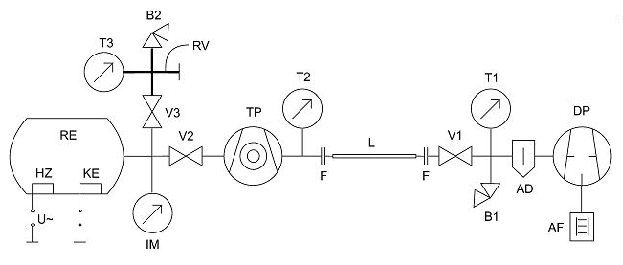
\includegraphics[width=.5\textwidth]{./img/apparatus.pdf}
	\caption[The apparatus]{The apparatus}
	\label{fig:apparatus}
\end{figure}
\autoref{fig:apparatus} shows the system of pumps and detectors used for the experiment. Following instruments and components are depicted:
\begin{table}[h!]
	\centering
	\begin{tabular}{ll}
		AD & adsorption trap	\\
		AF & exhaust filter	\\
		B1, B2 & vent valve\\
		DP & rotary vane pump (TRIVAC)	\\
		HZ & AC-heated evaporation boat	\\
		IM & ion gauge	\\
		KE & ball electrode (HV)	\\
		L & replacable connecting line	\\
		RE & recipient	\\
		RV & reference volume	\\
		T1, T2, T3 & thermal conductivity gauge (Thermovac)	\\
		TP & turbomolecular pump (TURBOVAC)	\\
		V1, V2, V3 & vacuum valve	\\
	\end{tabular}
\end{table}

\section{Mean Free Path}
The average distance that a particle can travel without interacting with another particle is called the mean free path.
It holds
\begin{equation}
	\lambda=\frac{1}{\sqrt{2}\pi n d^2}
\end{equation}
assuming a Maxwell-Boltzmann distribution.
Considering the ideal gas law $pV=nRT$, it is easy to see that the mean free path and pressure are reciprocal.
